\documentclass[a4paper,11pt]{article}
\usepackage{ctex}
\usepackage{fancyhdr}
\usepackage{graphicx}
\usepackage{float}
\usepackage{geometry}

\geometry{left=2.0cm, right=2.0cm, top = 3cm, bottom=3cm}
\pagestyle{fancy}
\fancyhf{}
\lhead{\leftmark}
\rhead{\rightmark}
\cfoot{\thepage}
\newcommand*{\dif}{\mathop{}\!\mathrm{d}}
\newcommand*{\e}{\mathop{}\!\mathrm{e}}

\title{阻尼振动与受迫振动实验}
\author{左京伟 \qquad 未央-电11 \qquad 2021012328}
\date{\today}


\begin{document}
\maketitle
% \tableofcontents
\begin{abstract}
    本实验的原理为阻尼振动和受迫振动的力学特性,借助波尔共振仪,探究阻尼振动、受迫振动以及共振的运动规律。实验分为三个部分:
    
    1. 观测不同阻尼对简谐振动的影响,了解阻尼振动。

    2. 分析受迫振动的基本规律,测试幅频特性和相频特性。

    3. 探究受迫振动的瞬态过程(振动系统在共振频率信号激励下的从静止到稳态的过程)。

    通过对于振动状态的观察,我了解同一个振子在不同阻尼状态和受迫状态下运动的差异与相似之处,掌握了振动系统的一般求解方法,并且知悉了描述振动系统损耗大小的参数——品质因数。

\end{abstract}

\section{实验仪器}
\paragraph{波尔共振仪}
    (如图 \ref{pic1})
    弹簧和圆形摆轮构成的待测振动系统,产生阻尼的电磁阻尼模块,产生激励的步进电机,用来测量相位差的有机玻璃转盘。
    \begin{figure}[ht]
        \centering
        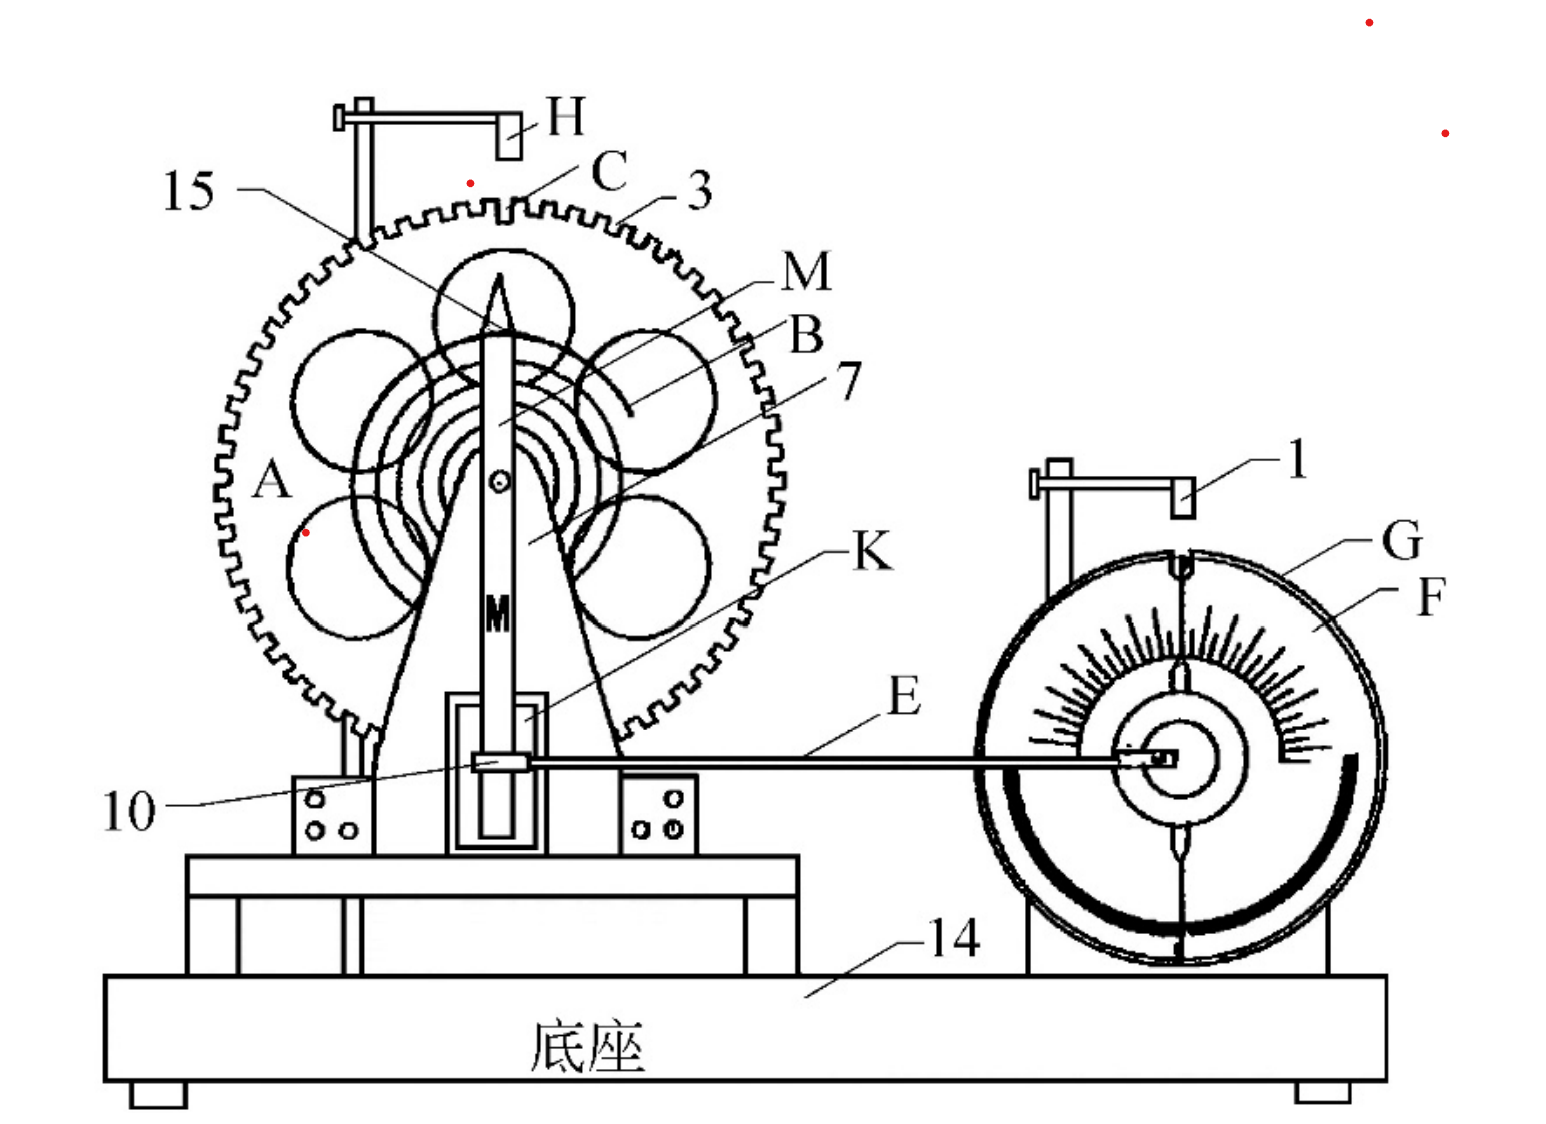
\includegraphics[scale=0.3]{Bohr.png}
        \caption{波尔共振仪}
        \label{pic1}
    \end{figure}
\paragraph{波尔共振实验箱}
    (如图 \ref{pic2})
    用于测量周期、调节阻尼大小、调节激励频率。
    \begin{figure}[ht]
        \centering
        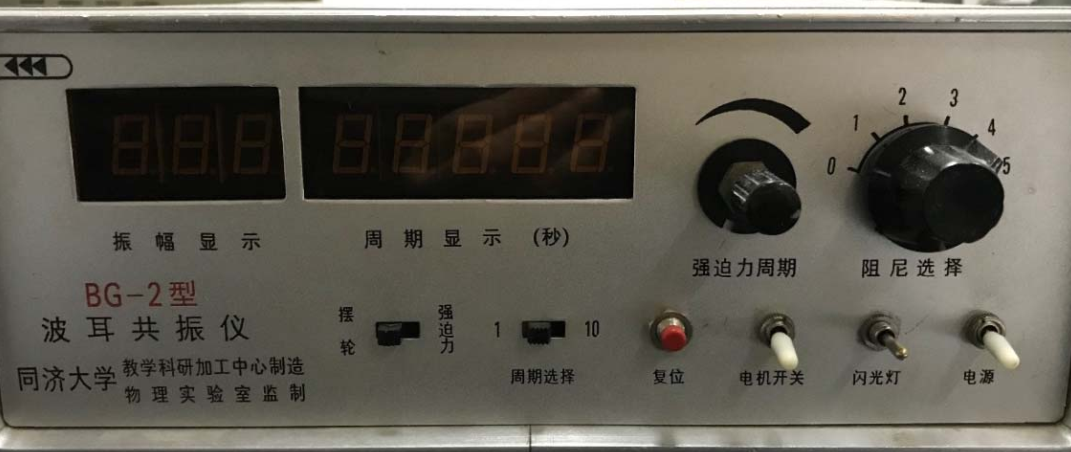
\includegraphics[scale=0.6]{box.png}
        \caption{波尔共振实验箱}
        \label{pic2}
    \end{figure}

\paragraph{仪器参数}
有机玻璃转盘:量程 $0^{\circ} \sim 180^{\circ}$ ,分度值$1^{\circ}$, 不确定度近似取为分度值的一半,即 $0.5^{\circ}$ .

波尔共振实验箱: 振幅有效量程:$0^{\circ} \sim 180^{\circ}$,分度值$ 1^{\circ}$,不确定度 $1^{\circ}$. 周期1档,量程$0.000 \sim  99.999s $ 分度值 $0.001s$,不确定度$0.002s$,周期10档,量程$0.000 \sim  99.999s $ 分度值 $0.001s$,每个周期不确定度$0.0002s$.

\section{实验内容}
    \subsection{观测有粘滞阻尼时的阻尼振动规律}
        \textbf{\romannumeral1. 理论部分}

        我们尝试从已经学过的无阻尼的振动的求解,推广至有阻尼的振动的求解。

        \textbf{无阻尼自由振动}
        
        摆轮受到弹簧的恢复力矩与摆轮偏离平衡位置的角度$ \theta $成正比,方向和$ \theta $相反,即

        \begin{equation}
            M = -k \theta
        \end{equation}

        设摆轮的转动惯量为$ J $,弹簧劲度系数为$ k $,由于弹簧质量相较于摆轮可以忽略不计,因此忽略弹簧的转动惯量。由此可列出摆轮转角$ \theta $的运动方程

        \begin{equation}
            J \frac{\dif^2 \theta}{\dif t^2} = -k \theta
        \end{equation}

        解得

        \begin{equation}
            \theta = \theta_0 \e^{i(\omega_0 t + \phi_0)}
        \end{equation}

        其中$ \theta_0 $为摆轮的初始振幅, $ \omega_0=\sqrt{\frac{k}{J}} $为自由振动的\textbf{固有角频率},$ \phi_0 $为初始相位。振动系统的总能量

        \begin{equation}
            E = E_k + E_p = \frac{1}{2}J\dot{\theta}^2 + \frac{1}{2}k\theta^2 = \frac{1}{2}k{\theta_0} ^2
            \label{eq: energy wrt amplitude}
        \end{equation}

        可以发现总能量和初始振幅的平方成正比,且机械能守恒。

        \textbf{阻尼振动}

        本实验的阻尼力是由电磁阻尼提供的,其大小和速度大小成正比,方向和速度方向相反,即

        \begin{equation}
            M_r = -\gamma \dot{\theta}
        \end{equation}

        阻尼振动系统动力学方程

        \begin{equation}
            J\frac{\dif^2\theta}{\dif t ^2} = -k\theta - \gamma \frac{\dif \theta}{\dif t}
        \end{equation}

        设阻尼系数
        
        \begin{equation}
            \beta = \frac{\gamma}{2J}
            \label{eq: beta}
        \end{equation}

        整理得到

        \begin{equation}
            \frac{\dif^2\theta}{\dif t^2} + 2\beta\frac{\dif\theta}{\dif t} + {\omega_0}^2 \theta = 0
            \label{eq: damped}
        \end{equation}

        是二阶线性齐次常微分方程。设特征根为$\omega$,代入可得

        \begin{equation}
            \omega^2 - 2i\beta \omega - {\omega_0}^2 = 0
        \end{equation}

        解得

        \begin{equation}
            \omega = i\beta \pm \sqrt{{\omega_0}^2 - \beta^2}
        \end{equation}
        
        因此方程(\ref{eq: damped})的通解即为

        \begin{equation}
            \theta = A\e^{i(\omega t + \phi)}
        \end{equation}

        观察发现,$\omega$中的$i\beta$项最终会产生一个指数衰减项,而后面根号内部的正负则会决定最后是否会是一个周期运动。因此我们有必要对于根号下的式子的正负进行讨论,由此把运动分为三种情况:
        \begin{enumerate}
            \item [a)] 过阻尼 $\beta > \omega_0$
            
            此时方程(\ref{eq: damped})的解为
            \begin{equation}
                \theta = \e^{-\beta t}(\theta_1 \e^{\sqrt{\beta^2-{\omega_0}^2}t}+\theta_2\e^{-\sqrt{\beta^2-{\omega_0}^2}t})
            \end{equation}

            可以发现这时系统主要表现为位移以指数规律缓慢\footnote{原因在于,两个项中第二个项很快衰减至0,主要是第一个项在起作用。而第一个项的指数因子为$\beta-\sqrt{\beta^2-{\omega_0}^2}$,这时一个比较小的数字。(相较于$\beta$而言)}衰减的运动特性。
            
            \item [b)] 临界阻尼
            
            此时方程(\ref{eq: damped})的解为
            \begin{equation}
                \theta = \theta_0 \e^{-\beta t}
            \end{equation}

            此时系统位移仍然呈现指数衰减的特性。振动系统接近平衡位置的时间最短。\footnote{衡量系统接近平衡位置的快慢可以使用时间常数$\tau = \frac{1}{\beta-\sqrt{\beta^2-{\omega_0}^2}}$去衡量。当$\omega_0$等于$\beta$的时候,时间常数$\tau$最小,因此最快接近平衡位置。}

            \item [c)] 欠阻尼
            
            此时方程(\ref{eq: damped})的解为
            \begin{equation}
                \theta = \theta_0 \e^{-\beta t}\cos(\omega_d t + \phi_0)
                \label{eq: underdamping angle expression}
            \end{equation}

            此时摆轮做振幅随时间指数衰减、周期保持恒定的振动。其角频率为$\omega_d=\sqrt{{\omega_0}^2-\beta^2}$.其值小于振子固有角频率$\omega_0$.换句话说就是周期更长。\footnote{这也与我们的直觉相符,受到阻力,振动会更加缓慢。}
        \end{enumerate}

        波尔振动仪提供的是欠阻尼,因此我们在本次实验中仅仅讨论欠阻尼的情况。

        \textbf{品质因数Q}

        在实际应用中,我们总是要关心系统阻尼的“大小”。那么,如何衡量所谓“大小”呢?仅仅看$\beta$的绝对值大小是没有意义的,因为不同系统的固有角频率不同。一个自然的想法就是系统每个周期损失了多少比例的能量。由此引出品质因数的定义:$2\pi$乘以振动系统存储的总能量$E$再除以一个周期内损失的能量$\Delta E$,即

        \begin{equation}
            Q = 2\pi\frac{E}{\Delta E}
        \end{equation}

        品质因数高,振动可持续的周期数多,相反地,品质因数低,振动就会更快地停止。

        对于本实验的摆轮-弹簧真东西套而言,当阻尼系数$\beta$较小的时候,可以认为振动系统的总能量$E$仍然与振幅的平方成正比\footnote{这是因为可以把一个周期内阻尼力做的功看成系统总能量的高阶无穷小。},式(\ref{eq: energy wrt amplitude})近似成立。由此可以推导低阻尼\footnote{本实验报告中,欠阻尼表示$\beta < \omega_0$的情况,而低阻尼表示$\beta \ll \omega_0$的情况,为防止混淆,特此注明。}振动系统的$Q$值

        \begin{equation}
            Q = 2\pi\frac{\frac{1}{2}k{\theta_n}^2}{\frac{1}{2}k{\theta_n}^2 - \frac{1}{2}k{\theta_{n+1}}^2}
              = \frac{2\pi}{1-(\frac{\theta_{n+1}}{\theta_n})^2}
              = \frac{2\pi}{1-\e^{-2\beta T_d}}
              \approx \frac{2\pi}{2\beta T_0}
              = \frac{\omega_0}{2\beta}
            \label{eq: quality}
        \end{equation}

        可见,与我们的直觉相符,振动系统的品质因数$Q$和阻尼系数$\beta$成反比。即阻尼越大,振动品质越低,振动越快趋于停止。

        \textbf{\romannumeral2. 实验部分}

        \textbf{A.0 $\beta$的量纲}

        由式(\ref{eq: beta})可知,$\beta$的量纲是$s^{-1}$.
        \\ \\
        \textbf{A.1 测量最小阻尼的阻尼系数$\beta$和系统固有角频率$\omega_0$}

        由式(\ref{eq: underdamping angle expression})可知,当$t=nT_d + t_0$时,摆轮的振幅为$\theta_n = \theta_0\e^{-\beta(nT_d+t_0)}$,发现这个式子是指数关系,直接拟合难度较大。所以采用两侧取对数的手段,得

        \begin{equation}
            \ln\theta_n = \ln\theta_0 - \beta t_0 - n\beta T_d
        \end{equation}

        每个周期测量一次振幅值$\theta_n$,再对$[\ln\theta_n , n ]$用最小二乘法拟合,斜率即为$-\beta T_d$.实验数据如下.\footnote{此处舍掉了原始数据中第一个数据,因为其偏差较大,初步考虑是由摆轮刚释放的第一个周期,光电门计数错误导致的。}

        \begin{figure}[ht]
            \centering
            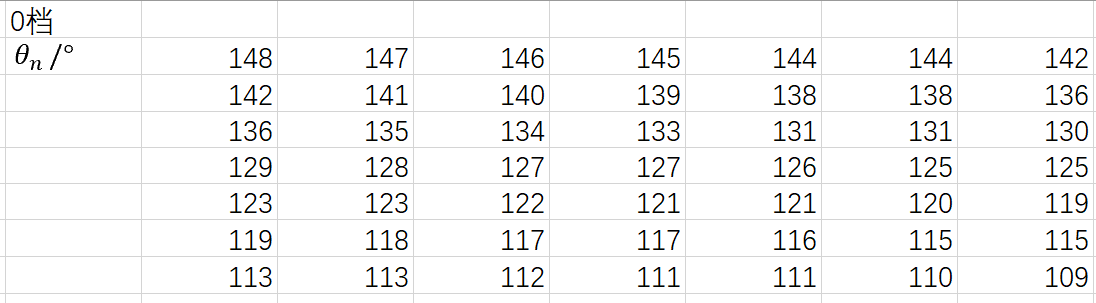
\includegraphics[scale=0.6]{无阻尼 角度数据.png}
            \caption{阻尼置于0档位的振幅数据}
        \end{figure}

        \begin{figure}[ht]
            \centering
            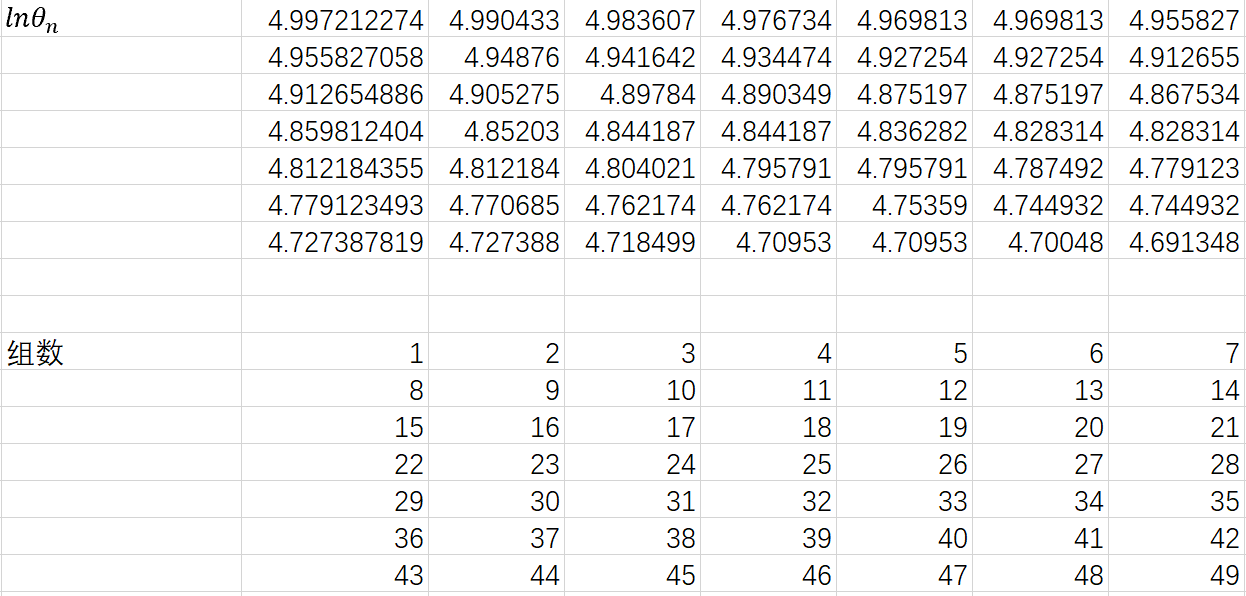
\includegraphics[scale=0.6]{无阻尼 拟合数据.png}
            \caption{阻尼置于0档位的待拟合的实验数据}
        \end{figure}

        利用Excel拟合,得
        $$
            k = -0.006321944
        $$
        $$
            s_k = 0.0000360311
        $$
        斜率不确定度\footnote{这里不考虑斜率的B类不确定度。}
        $$
            U_k = tinv(0.05, 49-2) \times s_k = 0.0000724853
        $$

        每10个周期测量一次$10T_d$,得到数据如下

        \begin{figure}[ht]
            \centering
            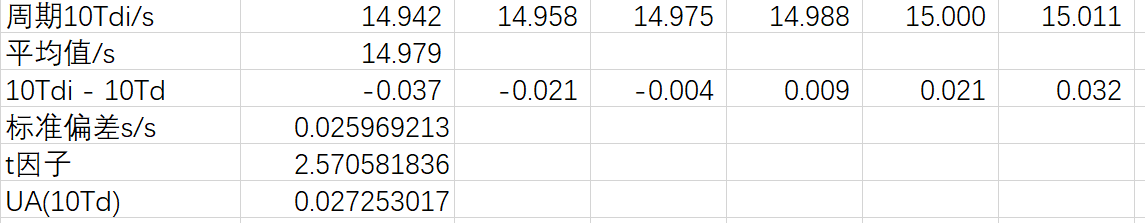
\includegraphics[scale=0.7]{无阻尼 周期.png}
            \caption{无阻尼振动的周期数据}
            \label{fig:label}
        \end{figure}

        所以$T_d$的A类不确定度$$U^A_{T_d} = 0.0027253017s$$

        $T_d$的B类不确定度为仪器误差限:$U^B_{T_d} = 0.0002s < \frac{1}{3} U^A_{T_d}$,满足微小分量判据。因此$T_d$的不确定度
        $$
            U_{T_d} = \sqrt{{U^A_{T_d}}^2 + {U^B_{T_d}}^2} \approx  U^A_{T_d} = 0.0027s
        $$

        由以上数据,我们可以计算0档的阻尼系数的量值
        $$
            \beta = -\frac{k}{T_d} = 0.004220538s^{-1}
        $$
        由不确定度的传递关系可知,$\beta$的不确定度满足如下关系
        $$
            \frac{U_\beta}\beta = \sqrt{(\frac{U_k}k)^2 + (\frac{U_{T_d}}{T_d})^2}
        $$
        由此得出
        $$
            U_\beta = 0.000049s^{-1}
        $$
        阻尼系数最终结果
        $$
            \beta = (0.004221 \pm 0.000049)s^{-1}
        $$
        \\ \\
        \textbf{A.2 用最小阻尼的阻尼系数$\beta$和振动周期$T_d$计算固有角频率$\omega_0$}
        $$
            \omega_d = \frac{2\pi}{T_d} = (4.195 \pm 0.008)s^{-1}
        $$
        由
        $$
            \omega_0 = \sqrt{{\omega_d}^2 + \beta^2}
        $$
        知$\omega_0$的不确定度
        $$
            U_{\omega_0} = \omega_0 \times \sqrt{(\frac{\omega_d}{\omega_d^2+\beta^2}U_{\omega_d})^2 + (\frac\beta{\omega_d^2+\beta^2}U_\beta)^2} = 0.008s^{-1}
        $$
        计算可知
        $$
            \omega_0 = (4.195 \pm 0.008)s^{-1}
        $$
        在实验精度内和$\omega_d$区别已经可以忽略。因此可以用0档的阻尼振动角频率$\omega_d$代替$\omega_0$.
        \\ \\
        \textbf{A.3 测量其他两种阻尼状态的振幅}

        数据处理方法和0档情况类似,因此略去不确定度的求解过程。因为振幅下降较快,数据采集的组数有所缩减。数据及其处理结果如下:

        \begin{figure}[ht]
            \centering
            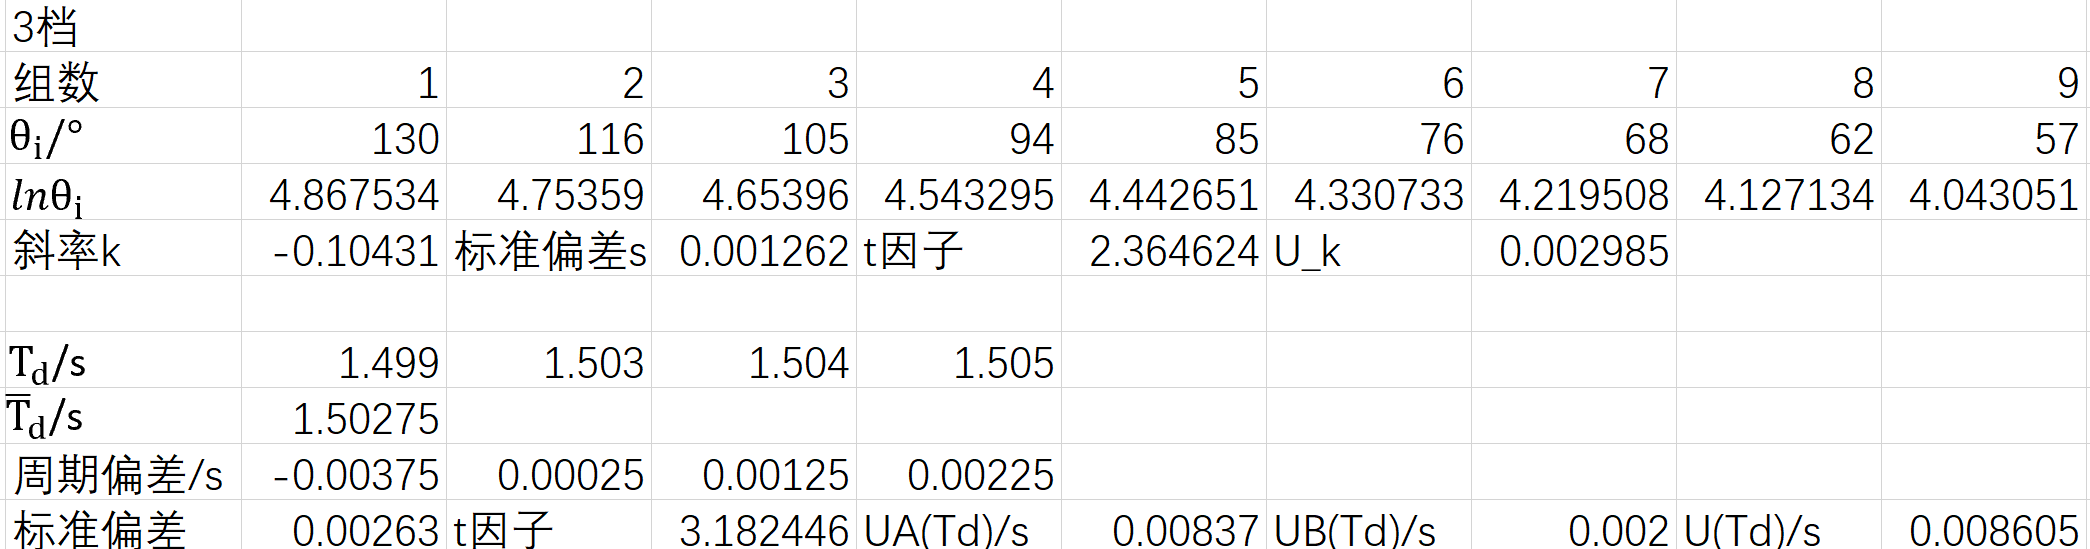
\includegraphics[scale=0.5]{3档阻尼 数据.png}
            \caption{3档阻尼实验数据及其处理结果}
        \end{figure}

        \begin{figure}[ht]
            \centering
            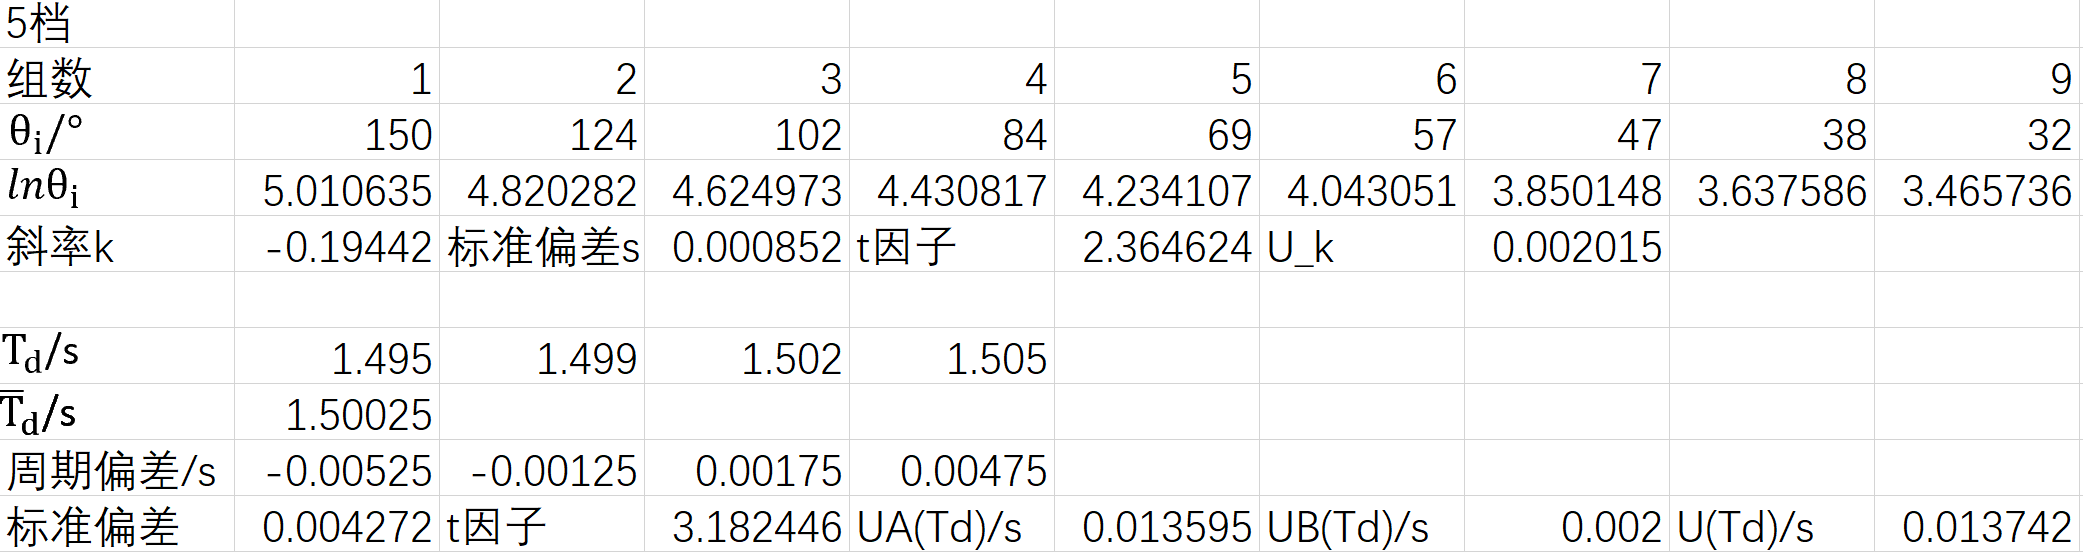
\includegraphics[scale=0.5]{5档阻尼 数据.png}
            \caption{5档阻尼实验数据及其处理结果}
        \end{figure}

        最终结果:

        3挡状态下
        $$
            \beta_3 = (0.0694 \pm 0.0020)s^{-1}
        $$

        5挡状态下
        $$
            \beta_5 = (0.1296 \pm 0.0018)s^{-1}
        $$
        \\ \\
        \textbf{A.4 利用不同阻尼状态下的阻尼系数$\beta$计算品质因数$Q$}
        \begin{enumerate}
            \item 0档阻尼:

            由此前数据及式(\ref{eq: quality})知
            $$
                Q = \frac{\omega_0}{2\beta} = 496.9345536
            $$
            由不确定度的传递关系可知
            $$
                \frac{U_Q}Q = \sqrt{(\frac{U_{\omega_0}}{\omega_0})^2 + (\frac{U_\beta}\beta)^2}
            $$
            所以求出
            $$
                U_Q = 5.840147
            $$
            最终结果
            $$
                Q = 496 \pm 6
            $$
            \item 3档阻尼
            
            求解过程类似,此处省略过程,给出最终结果
            $$
                Q = 30.1 \pm 0.9
            $$
            \item 5档阻尼
            
            求解过程类似,此处省略过程,给出最终结果
            $$
                Q = 16.16 \pm 0.20
            $$
        \end{enumerate}
        
    \subsection{分析振动系统受迫振动的基本规律}
    \textbf{\romannumeral1. 理论部分}

        弹簧振动系统在角频率为$\omega$,振幅为$A_D$的简谐激励下,运动方程将变为
        \begin{equation}
            \frac{\dif^2 \theta}{\dif t^2} + 2\beta \frac{\dif \theta}{\dif t} + \omega_0^2 \theta = \omega_0^2 A_D\cos(\omega t)
        \end{equation}

        欠阻尼情况下,通解为
        \begin{equation}
            \theta = \theta_0 \e^{-\beta t} \cos (\sqrt{\omega_0^2 - \beta^2}t + \phi_0) + \theta_m \cos(\omega t - \phi)
            \label{eq: 受迫振动通解}
        \end{equation}

        发现通解中前一项随着时间增加衰减至0,后一项是稳态运动解。

        稳态解的振幅
        \begin{equation}
            \theta_m = \frac{\omega_0^2 A_D}{\sqrt{(\omega_0^2 - \omega^2)^2 + (2\beta\omega)^2}}
            \label{theta}
        \end{equation}
        相位差
        \begin{equation}
            \phi = \arctan \frac{2\beta\omega}{\omega_0^2-\omega^2}
            \label{phi}
        \end{equation}
        无论什么情况,总有$0<\phi<\pi$.这表明,受迫振动系统振动相位总是落后于强迫力。

        \textbf{B.1 推导共振频率以及共振处振幅最大值的表达式}

        $\theta_m$达到最大的一个必要条件是
        \begin{equation}
            \frac{\dif \theta_m}{\dif \omega} = 0
        \end{equation}
        由此式解出,当$0<\beta<\omega / \sqrt2$时
        \begin{equation}
            \omega = \sqrt{\omega_0^2 - 2\beta^2}
        \end{equation}
        易验证此时$\theta_m$确实取到极大值,也即最大值。
        代入 式(\ref{theta})和 式(\ref{phi})可得,系统共振时的稳态振幅
        \begin{equation}
            \theta^*_m = \frac{A_D\omega_0^2}{2\beta\sqrt{\omega_0^2-\beta^2}}
        \end{equation}
        和稳态相位差
        \begin{equation}
            \phi^* = \arctan \frac{\sqrt{\omega_0^2-2\beta^2}}\beta
        \end{equation}
        在低阻尼情况下($\beta \ll \omega_0$),有近似解
        \begin{equation}
            \omega = \omega_0\sqrt{1-2(\frac\beta{\omega_0})^2} \approx \omega_0
        \end{equation}
        \begin{equation}
            \theta^*_m = \frac{A_D\omega_0}{2\beta} = A_D Q
        \end{equation}
        \begin{equation}
            \phi^* = \arctan \frac{\omega_0}{\beta} = \arctan 2Q
        \end{equation}
    ~\\
    \textbf{\romannumeral2. 实验部分}

        \textbf{B.1 共振频率,振幅最大值和相位差的表达式,推导在弱阻尼状态下的共振频率}

        见上理论部分。

        \textbf{B.2判断受迫振动达到稳态的方式}

        连续5次周期测量相等。

        \textbf{B.3 测定幅频特性和相频特性}

        阻尼档位分别置于3档和5档\footnote{此处选择的档位和A.3中一致。},打开步进电机,调节电机频率,通过闪光灯观察相位差,用实验箱测量周期和振幅,得到实验数据如图(\ref{fig: 幅频相频数据})所示。

        \begin{figure}[ht]
            \centering
            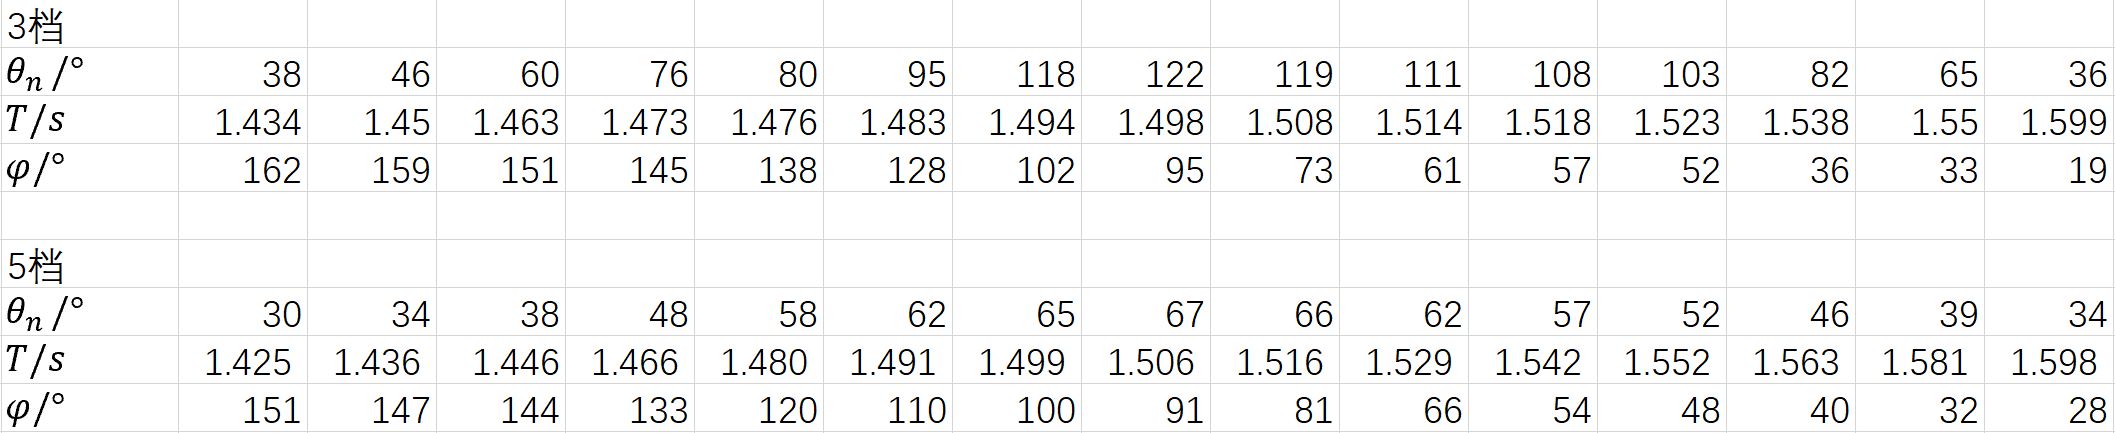
\includegraphics[scale=0.5]{幅频相频数据.png}
            \caption{受迫振动振幅和相位差的实验数据}
            \label{fig: 幅频相频数据}
        \end{figure}

        \textbf{B.4 绘制幅频特性曲线和相频特性曲线}

        绘制出幅频特性曲线,如图(\ref{fig: 幅频特性曲线})所示。

        \begin{figure}[ht]
            \centering
            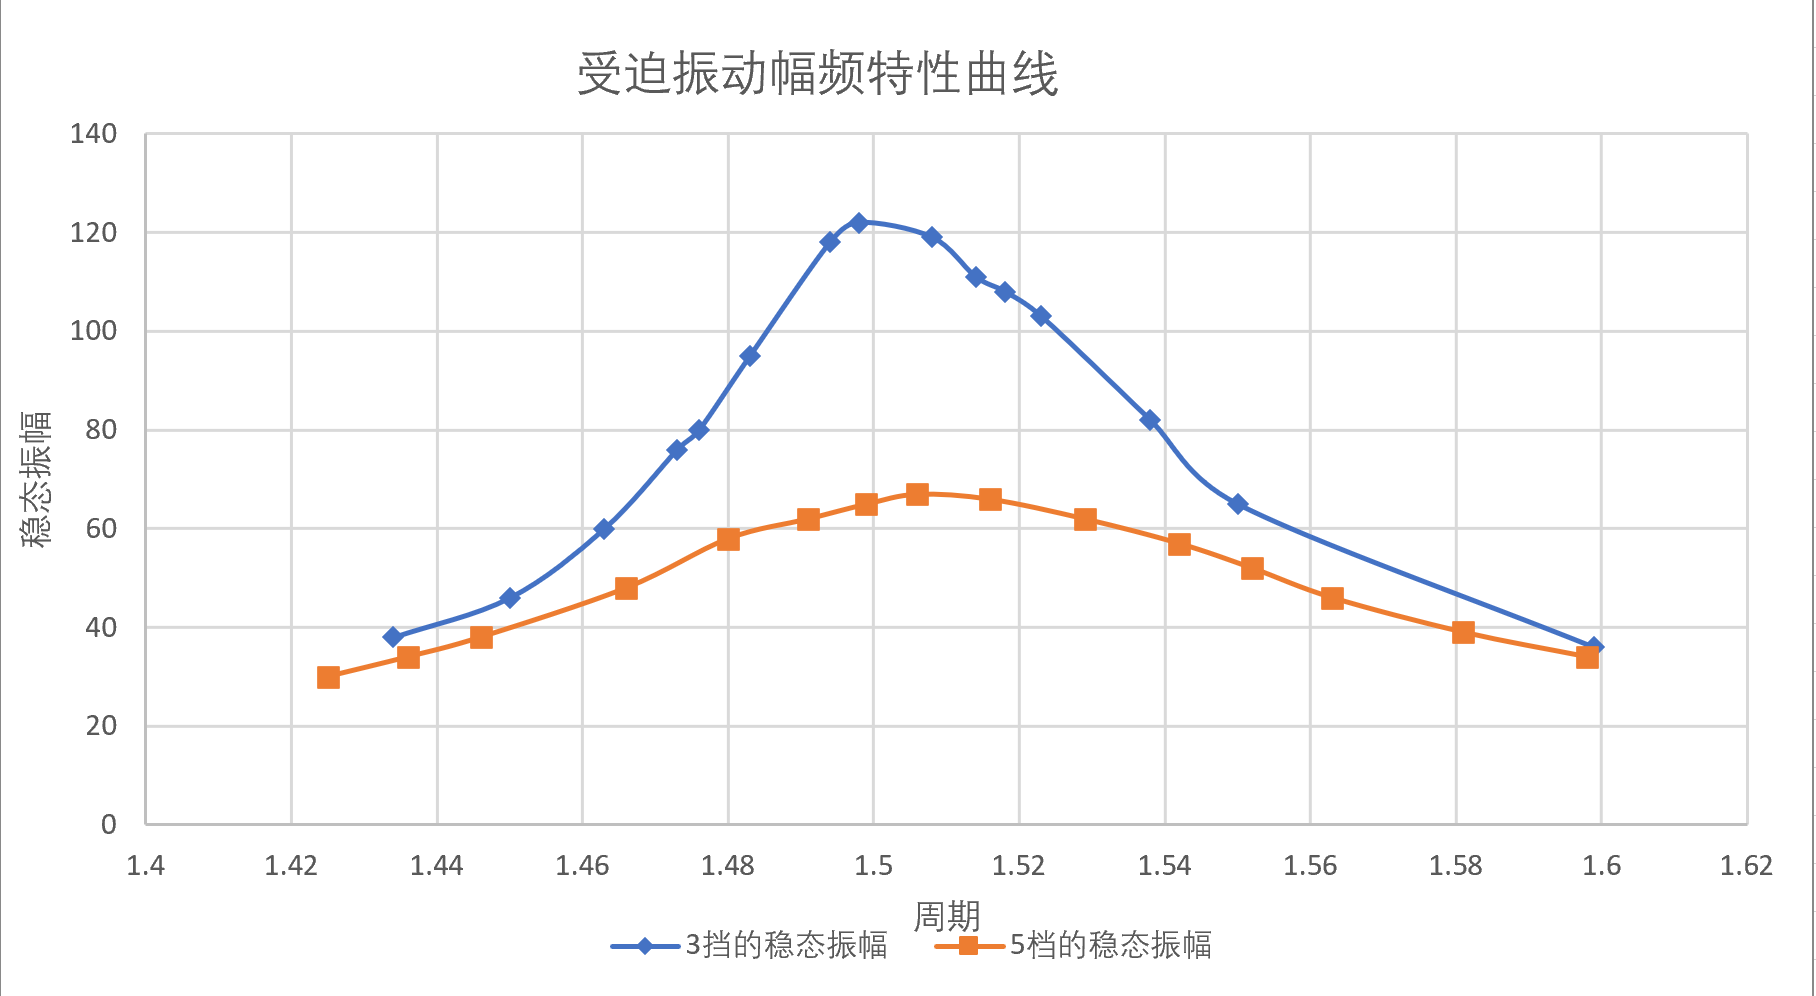
\includegraphics[scale=0.5]{幅频特性曲线.png}
            \caption{幅频特性曲线}
            \label{fig: 幅频特性曲线}
        \end{figure}

        和相频特性曲线,如图(\ref{fig: 相频特性曲线})所示

        \begin{figure}[ht]
            \centering
            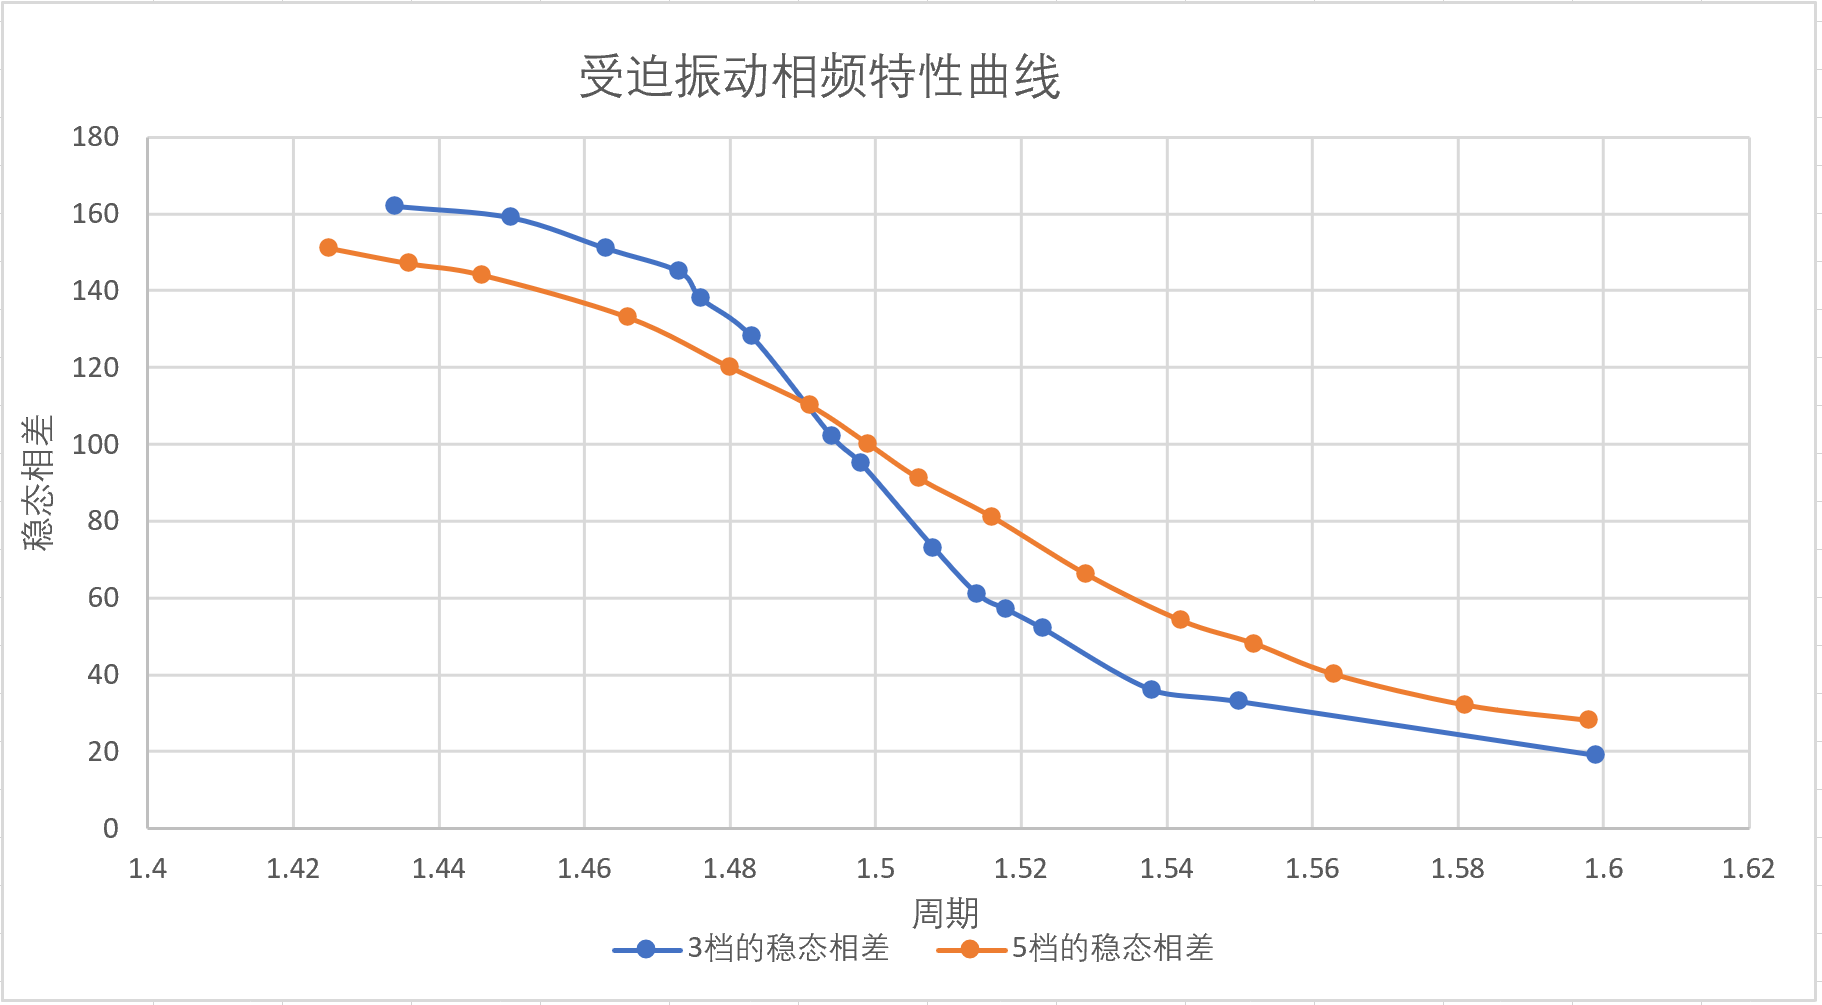
\includegraphics[scale=0.5]{相频特性曲线.png}
            \caption{相频特性曲线}
            \label{fig: 相频特性曲线}
        \end{figure}

        理论计算出,3档阻尼的理论共振周期
        $$
            T_3 = \frac{2\pi}{\sqrt{\omega_0^2-2\beta^2}}\Bigg|_{\beta = 0.0694s^{-1}} =  1.498s
        $$

        5档阻尼的理论共振周期
        $$
            T_5 = \frac{2\pi}{\sqrt{\omega_0^2-2\beta^2}}\Bigg|_{\beta = 0.1296s^{-1}} =  1.499s
        $$

        和从图中读出的最大振幅位置处的强迫力周期能够较好地符合。

        \textbf{B.5 由幅频特性曲线计算品质因数Q}

        由理论分析可知,在低阻尼情况下,品质因数$Q$可如此表示

        \begin{equation}
            Q \approx \frac{\omega_r}{|\omega_+-\omega_-|}
        \end{equation}

        其中,$\omega_r$为振幅最大时对应的角频率,$\omega_\pm$为振幅等于$\frac{\sqrt{2}}2$倍振幅最大值对应的两个角频率值。

        从图中读数,得到

        3挡
        $$
            T_r = 1.499s
        $$
        $$
            T_- = 1.481s
        $$
        $$
            T_+ = 1.532s
        $$
        计算得出品质因数
        $$
            Q = \frac{T_-T_+}{T_r|T_+-T_-|} = 30 \pm 1
        $$
        
        5挡
        $$
            T_r = 1.507s
        $$
        $$
            T_- = 1.466s
        $$
        $$
            T_+ = 1.559s
        $$
        计算得出品质因数
        $$
            Q = \frac{T_-T_+}{T_r|T_+-T_-|} = 16 \pm 1
        $$
        和A.4中比较,发现在误差范围内符合得很好,这说明了用幅频特性曲线计算品质因数的合理性。

    \subsection{探究受迫振动的瞬态过程}
        \textbf{C.1 测试3档阻尼下系统受迫振动的瞬态过程,绘制振幅-时间曲线并将理论和实际相对比}

        将阻尼档置为3档,将摆轮拨至平衡位置,并让其静止。此时打开电机开关,使摆轮开始振动,同时立刻开始记录振幅和周期数据,数据见图(\ref{fig: 受迫振动瞬态数据})。

        \begin{figure}[ht]
            \centering
            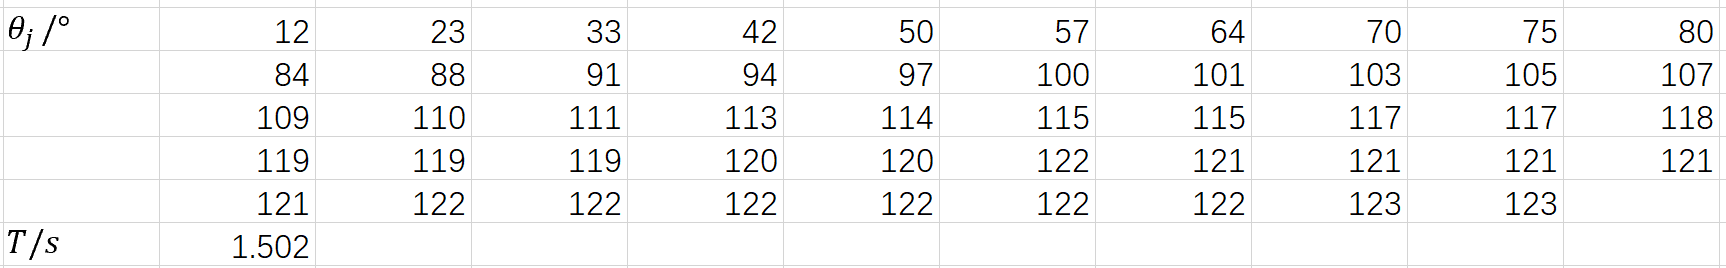
\includegraphics[scale=0.6]{受迫振动瞬态数据.png}
            \caption{受迫振动瞬态振幅即周期数据}
            \label{fig: 受迫振动瞬态数据}
        \end{figure}

        并由此绘制出振动系统振幅随着时间变化的曲线,如图(\ref{fig: 振幅曲线})所示。

        \begin{figure}[ht]
            \centering
            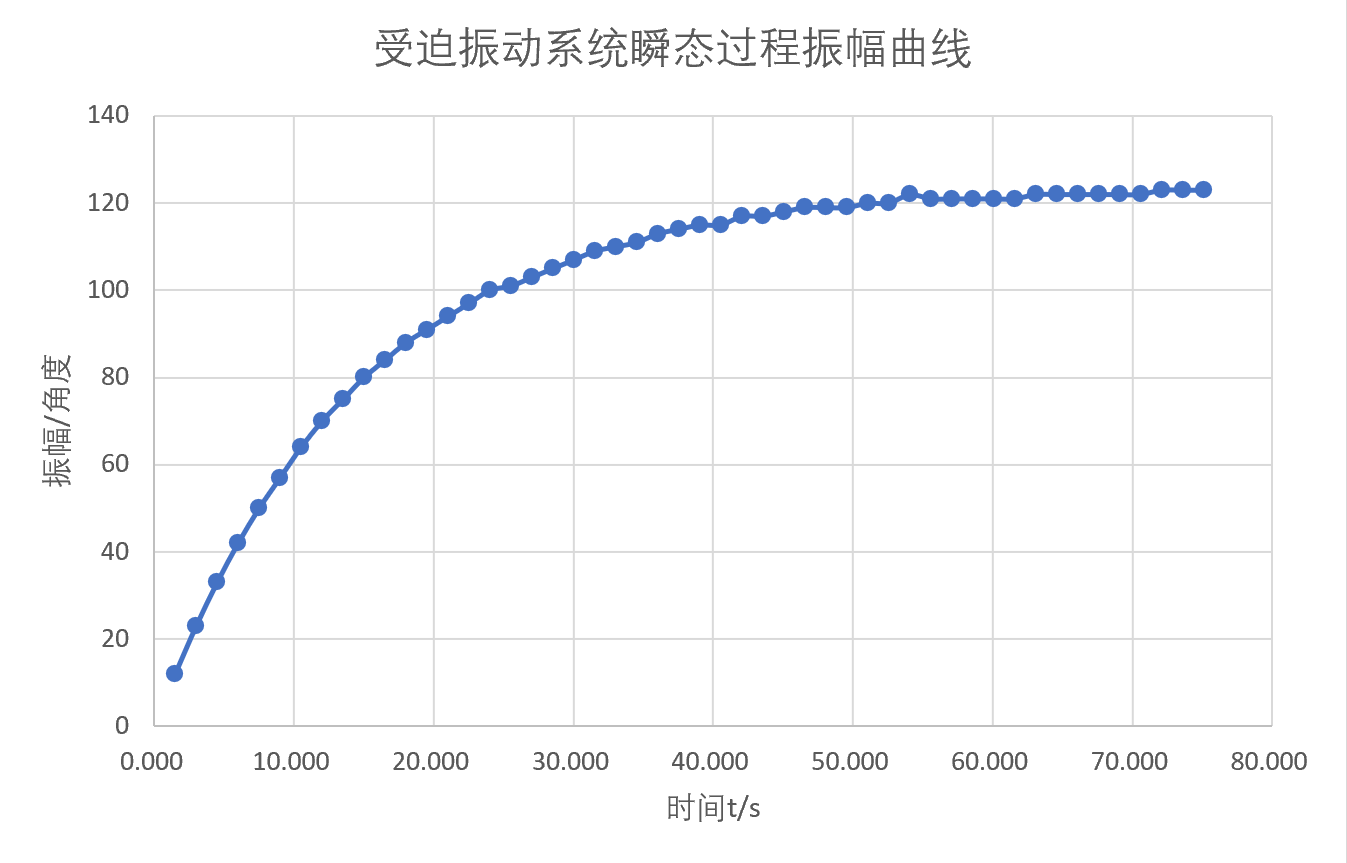
\includegraphics[scale=0.7]{受迫振动瞬态振幅曲线.png}
            \caption{受迫振动瞬态振幅曲线}
            \label{fig: 振幅曲线}
        \end{figure}

        由式(\ref{eq: 受迫振动通解}),代入初始值$\theta(0) = 0$和$\dot{\theta}(0) = 0$,结合低阻尼近似\footnote{这种近似的合理性在于,A实验已经测定,3档阻尼的$\beta = (0.0694 \pm 0.0020)s^{-1} $,和$\omega_0 = (4.195 \pm 0.008)s^{-1}$对比可知,数量级相差2倍。},可以得到
        \begin{equation}
            \theta_0 = -\theta_m
        \end{equation}
        再代回式(\ref{eq: 受迫振动通解}),得到
        \begin{equation}
            \theta = \theta_m(1-\e^{-\beta t})\sin\omega_0t
        \end{equation}
        可知振幅的表达式
        \begin{equation}
            \theta_{max} = \theta_m(1-\e^{-\beta t})
        \end{equation}
        将理论值绘制出曲线,和实际振幅绘制在一幅图中,如图(\ref{fig: 受迫理论和实际})所示。
        
        \begin{figure}[ht]
            \centering
            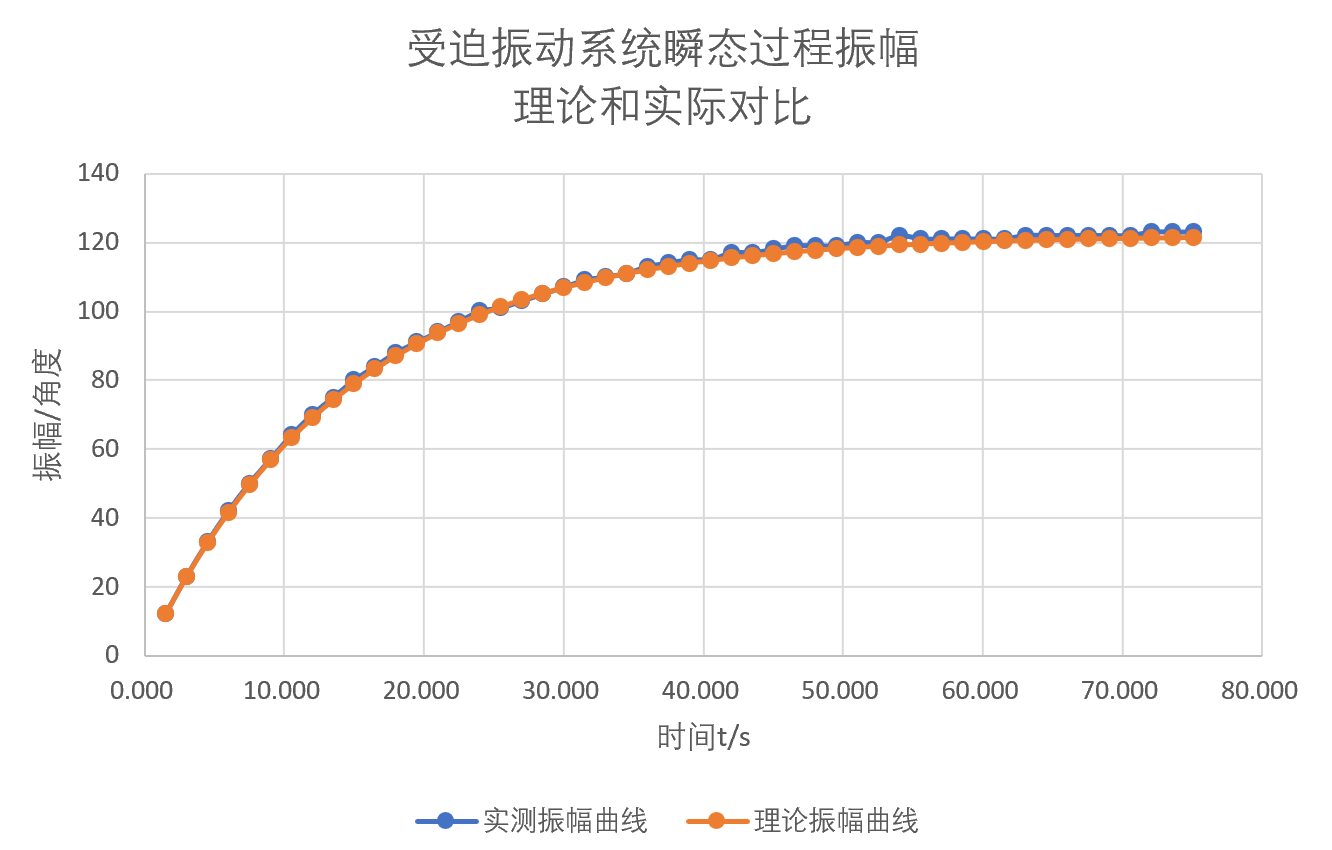
\includegraphics[scale=0.7]{受迫振动瞬态振幅理论和实际对比曲线.png}
            \caption{受迫振动瞬态振幅理论和实际对比曲线}
            \label{fig: 受迫理论和实际}
        \end{figure}

        可以看出,理论曲线和实测曲线在误差范围内符合的程度是非常之高的。
        ~\\~\\
        \textbf{C.2 推导振动系统达到稳态之后电机在一个周期内提供的平均输入功率}
            达到稳态之后,系统总机械能维持恒定不变。因此,一个周期内,电机对系统做功等于系统克服阻尼力做的功,即
            \begin{eqnarray}
                W_{motor} = W_{resistance} = \int M_r \dif \theta
                
            \end{eqnarray}
\end{document}